\documentclass[conference]{IEEEtran}

\IEEEoverridecommandlockouts
\usepackage{cite}
\usepackage{amsmath,amssymb,amsfonts}
\usepackage{algorithmic}
\usepackage{graphicx}
\usepackage{textcomp}
\usepackage{xcolor}
\usepackage{fancyhdr}
\usepackage{lipsum}

\def\BibTeX{{\rm B\kern-.05em{\sc i\kern-.025em b}\kern-.08em
    T\kern-.1667em\lower.7ex\hbox{E}\kern-.125emX}}
    
\fancypagestyle{firstpagefooter}{%
  \fancyhf{}
  \renewcommand\headrulewidth{0pt}
  \fancyfoot[R]{IOT Challenges: Functional Safety, Hamm-Lippstadt Hochschule}
}

\pagestyle{empty}

\bibliographystyle{IEEEtran}

\begin{document}
\title{IOT Challenges: Functional Safety}

\author{\IEEEauthorblockN{Vytaras Juraska}
\IEEEauthorblockA{\textit{Electronics Engineering (7\textsuperscript{th} Semester)} \\
\textit{Hamm-Lippstadt Hochschule}\\
Lippstadt, Germany \\
vytaras.juraska@stud.hshl.de}
}

\maketitle

\begin{abstract}
in this paper main focus is emphasizing the importance of functional safety in the field of Internet Of Things (IOT), while also analyzing the today's standardised requirements, which each IOT device has to follow.
\end{abstract}

\thispagestyle{firstpagefooter}

\section{Introduction to Internet of Things (IOT)}

The Internet of Things (IoT) \cite{alzahrani_sensing_2017} is upcoming and constantly evolving technology which allows different devices (which in IoT field are considered as “things”) to communicate through the Internet connection. Currently, IoT is known to use more and more of Artificial Intelligence techniques, which helps processing data gathered by different sensors and predict the next action accordingly. In terms of various fields, where IoT is being widely implemented, are as follows: manufacturing, agriculture, education, commercialization, smart homes, auto cars, medical and so on. 

In fact, IoT is such a vastly adapted technology, that general purpose IoT technologies for some cases are not suitable enough, hence various of application specific IoT fields are in constant development (e.g. Internet of Medical Things (IoMT), Internet of Underwater Things (IoUT) along with others) \cite{ang_application_2019}. For instance, a specific IoT for environmental water monitoring would have different requirements from a specific IoT for medical monitoring, which would require much higher and more precise requirements for real-time data transfer and security.

Another important topic about IoT is its safety and security, which at current state is exposed in concerning levels \cite{hayakawa_proposal_2018}. Internet already introduces a magnitude of security issues, such as cyber-attacks, malware, etc.
One of the examples in bad security practice happened in 2016 with an insulin pump. According to the references \cite{hayakawa_proposal_2018}, the specified device users experienced impersonation issues by third party, which had the possibility to cause malfunction of the equipment, leading to a possibility of risking a human life, since it is, in fact, a medical device, which is crucial to some users. Surprisingly, manufacturers did not take any actions, rather advised users in correct usage of the device. In this case, this should not be the case - human error handling a device, which is meant for an average patient, can not lead to device failure. Thus, manufacturers must apply specific Secure by Design practices, which would take functional safety seriously already from the design phase of development.

\subsection{General Applications of IOT}

\subsubsection{Personal}

This would include personal health, such as\footnote{https://ordr.net/article/iot-healthcare-examples/}:
\begin{itemize}
    \item Remote Patient Monitoring - one of the most common applications, monitoring vital variables of a human body like heart rate, blood pressure, temperature and so on. Generally, its purpose is for patients, who can not visit a healthcare facility - vitals could still be monitored and medical advice could be handled accordingly. Automatic analyzing helps to inform healthcare professionals about an upcoming problem, which creates an opportunity to stop an upcoming issue before the situation gets worse;
    \item Glucose Monitoring - for a significant amount of people across the world with diabetes, glucose monitoring has been not the most simplest process. Traditionally, it had to be tracked and checked manually, hence the patients received the results only after executing the initial manual test, which creates problems for people with widely fluctuating glucose levels. Current IoT device allows for continuous, automatic monitoring of glucose, which can also alert the patient, if the levels are too low and track the data automatically\footnote{https://www.niddk.nih.gov/health-information/diabetes/overview/managing-diabetes/continuous-glucose-monitoring}.
    \item Hand Hygiene Monitoring - a device, which informs a user upon the inspection, if their hands are clean. This is practical especially at unique times like the current crisis situation, where hand cleanliness is an important aspect. Traditionally, there has not been a quick and effective way to check it automatically, but this solution with the availability of sensors and their IoT communication, can achieve acceptable results\footnote{https://biovigil.com/}.
\end{itemize}

There are many various examples of application, but generally, personal use can extend even to ways of social interaction, hence the possibilities in this field are limitless.

\subsubsection{Home}

Electronic appliances integrated with IoT redefine communication between user and devices. Every electronic appliance, such as lights, air conditioning, security cameras, refrigerator, oven and so forth can be connected to the internet quite simply. Integrating a smartphone into the scenario and the customer now can remotely control almost any electronic appliance there is. 

In one of the references \cite{ramson_applications_2020}, authors mention some application examples:

\begin{itemize}
    \item Ambient intelligence-based lightning system has an integrated intrusion detection, which will detect intrusion and give alert to the nearby police station, by acquiring exact geographical location;
    \item Gas or smoke detection system, which sends an e-mail or SMS to fire department.
\end{itemize}

Home environment field has also many benefits from the IoT integration to everyday technology.

\subsubsection{Industrial}

Not surprisingly, the industry also benefits greatly from the technology of IoT, since most industrial machinery are using a bulk of various sensors, with which communication is crucial\footnote{https://nexusintegra.io/7-industrial-iot-applications/}. Here are some areas of application, as an example of where this technology is being used and for what purpose:

\begin{itemize}
    \item Remote automated equipment management and monitoring is one of the main Industry IoT use-cases, which allows to have a centralized system, to execute a crucial task of equipment maintenance. The remote characteristic also implies, that this technology can be adapted to maintain more than one geographical location at a time;
    \item Predictive maintenance is a system integrated with IoT, which sends alerts, when the machinery are in dire need of maintenance before a crisis occurs.
    \item Quality control is another massive application, from raw materials to the built product - with the help of various sensors, AI and precise real-time calculations IoT technologies help analyze the product, record each analysis of the product and inform engineers at which part the product maintain quality, and if error happened, at which point it was detected.
\end{itemize}
\section{Introduction to Functional Safety}
As mentioned before, IoT is a field, which has accumulated big interests in various of applications. Some applications are crucially important, where a single failure could cause undesirable and devastating results, good example was given, referring the insulin pump device. Generally, IoT is being implemented in a lot of fields, so having a standardised method of risk-free products in every application is a complicated matter, since every application, as mentioned before, can be so unique, that the general requirements might not fit the product as much as specific requirements.

To understand how complex risk prevention implementing IoT is - in the reference \cite{tomur_sok_2021} a topic of security and functional safety specifically in industrial IoT applications is investigated. These two terms have shared goals of preventing a product or a system from risks, but they do have unique differences, which have to be understood.

\subsection{Meaning of Functional Safety}

The word safety is "defined as the state of being free from unacceptable risk, which causes direct or indirect harm to human health, environment or property" \cite{tomur_sok_2021}, hence the importance of safety is prevention from physical harm. Regarding functional safety, it is a term, which mostly relates to software applications, where correct operation of the system prevents from physical harm at acceptable levels, by reassuring successful communication and control, when it is required.

\subsection{Meaning of Security}

Security risks are concerning on deliberate malicious intents, where when exploited - vulnerabilities can affect both physical and cyber world.

\subsection{Comparison between Safety and Security}

Functional safety is focusing on protecting purely physical world assets (human health and life, environment and equipment) from dangers of Operational Technology (OT) malfunctions, while Information Technology (IT) security is all about protecting the information of all IT related assets. Previously security and safety were two different subjects, being operated in their own separate domains, but generally, these two systems have a strong connection with each other (Figure \ref{OTIT}).

\begin{figure}[htbp]
\centerline{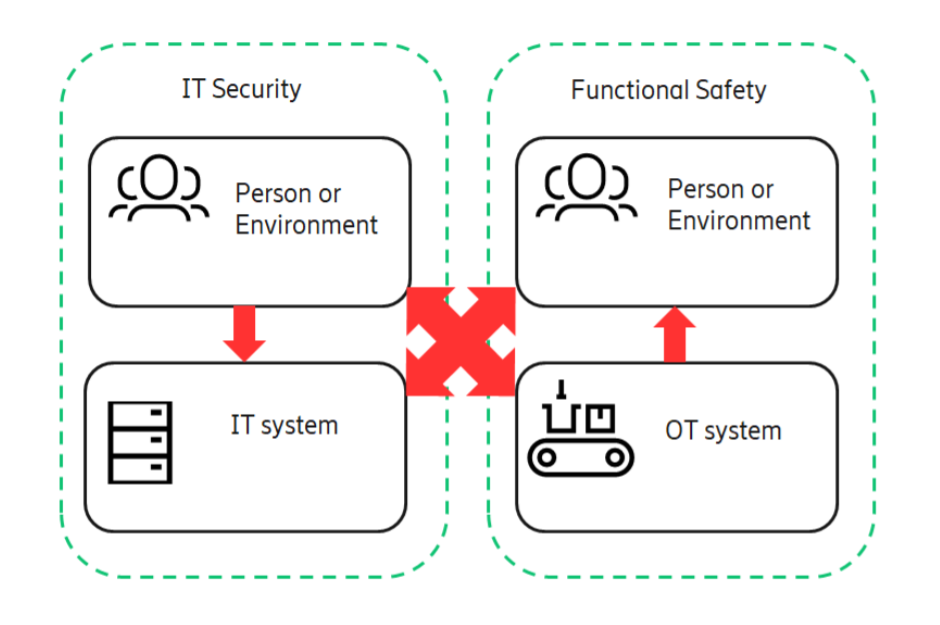
\includegraphics[scale=.45]{OT_IT.png}}
\caption{Inter-connectivity of OT and IT \cite{tomur_sok_2021}}
\label{OTIT}
\end{figure}

There are cases, especially in IoT applications, where bypassed security of IT can directly affect OT. For an example - Triton Malware, a malicious attack in 2017, which targeted safety of oil and gas petrochemical facilities, which ended up in putting systems into emergency stop. Fortunately, the outcome was just lost availability of equipment, but this is a good example of how important it is to consider both risk-preventing systems, when developing and designing security and safety.

\section{Characteristics of Functional Safety}

Knowing, that functional safety focuses for machinery and equipment hazard control, couple of important characteristics have to be analyzed to get a wider understanding of this specific field.

\subsection{Machinery Safety Functions}

Mostly, the machinery is implemented with a detection system, which checks if there is a person on any other environmental asset, which has to be insured with risk-prevention. One of the examples of it is an entrance door with an interlock, for which to open, the safety relay has to check the robot safety system, if it is safe for someone to enter the area (Figure \ref{Interlock}). This example would provide suitable level of risk reduction in terms of functional safety and also satisfy such requirements as safety reaction time, since the door would not open, if a threat is a possibility.

\begin{figure}[htbp]
\centerline{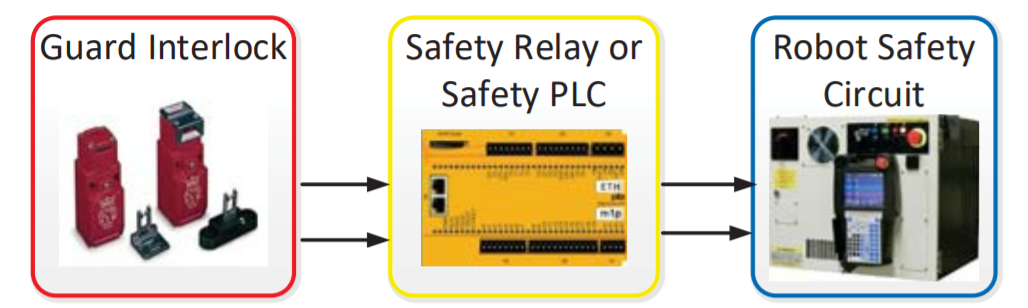
\includegraphics[scale=.4]{Machinery_FuSa.png}}
\caption{Safety block functions in machinery applications \cite{robinson_living_2019}}
\label{Interlock}
\end{figure}

\subsection{Safety Integrity Level}

To compare, analyze and understand the amount of required functional safety, specific levels have to be considered, which would help creating a specific goal for safety, to be able to achieve better quality of safety. In the case of Safety Integrity Level the variable in consideration is average frequency of dangerous failure per hour, which is defined as probability of failure on demand (PFD). Two international different standards cover the requirements of safety, which help analyze this variable: ISO 13849 and IEC 61784.

\section{Standardised Requirements}

When it comes to safety, standardisation is a way to ensure, that majority of companies, factories and their products would be provided with the needed protection. Of course it is not an easy task - making a standard system, which would be sufficient, applicable and optimised for all the fields in question. Functional safety is no exception, it has a couple of main standards, which are: ISO 13849 and IEC 61508.

\subsection{IEC 61508}

In the context of industrial applications (to distinguish from aerospace and military applications) a major initiative has been focused on IEC 61508 and this standard is
emerging as a key international standard in many industrial sector. Overall title of this standard is "Functional safety of electrical, electronic and programmable electronic (E/E/PE) safety-related systems" and there are 8 general main parts of the document itself \cite{bell_introduction_nodate}:

\begin{itemize}
    \item (Part 0) Functional safety and IEC 61508;
    \item (Part 1) General Requirements;
    \item (Part 2) Requirements for electrical, electronic and programmable electronic systems;
    \item (Part 3) Software Requirements;
    \item (Part 4) Definitions and abbreviations;
    \item (Part 5) Examples of methods for the determination of safety-integrity levels;
    \item (Part 6) Guidelines on the application of Parts 2 and 6;
    \item (Part 7) Overview of techniques and measures.
\end{itemize}

In terms of requirements, only described in parts 1, 2 and 3. Also, parts 1, 2, 3 and 4 are describing basic IEC safety applications.

\subsubsection{Influence and Usage}

IEC 61508 functions both as a stand-alone standard and can also be used as the basis for sector and product standards. So far it has been used in the process and machinery sectors and is being used to develop a standard of power drive systems - electrical or hydraulic power converting into mechanical motion. But mainly IEC 61508, as a standalone standard, influences overall E/E/PE (Electrical/Electronic/Programmable Electronic) safety related systems:

\begin{itemize}
    \item Definition of E/E/PE safety related general requirements, where no application sector or product standards exist and also where they are not applicable;
    \item Applied for and used by E/E/PE component suppliers;
    \item Applied for and used by system builders, in order to meet specifications for E/E/PE safety related systems.
    \item Defines maintenance by design safety integrity for E/E/PE safety related systems.
\end{itemize}

IEC 61508 is also used to provide technical framework for product fulfilment of standards and requirements and can be used by users, who specify requirements in terms of safety functions. And lastly, IEC 61508 is used for carrying out assessments of safety lifecycle activities.

\subsubsection{Strategy to Achieve Functional Safety}

IEC 61508 focuses on three safety lifecycles: software safety, E/E/PE safety and overall safety. So in order to achieve the required safety integrity level, this standard adopts the overall lifecycle as the technical framework, which is used, as stated before, to validate product fulfilment of standards, including IEC 61508. Overall lifecycle includes risk measures for safety related systems, such as E/E/PE, external risk reduction facilities and other technology systems.

Concerning E/E/PE and software lifecycles, they define simplified views of reality. Also activities, relating the management of functional safety assessments are not shown in overall, E/E/PE and software lifecycles, this was done in order to simplify the complexity, however, definition of such activities are required, when IEC 61508 is applied.

\subsubsection{Lack of Safety Example}

Studies were done, to support the requirement of overall safety lifecycle. One of them is done by Health and Safety Executive (1995), where an analysis of accidents and incidents involving safety related systems was done. In the figure \ref{safety_graph} a graph is shown which represents primary causes of failure by each lifecycle phase.

According to the study, most control system failures were caused by insufficient definition of specifications. Some had lack of hazard analysis, some had no specification concerning critical failures. However, in reality control systems need to be reviewed in each lifecycle phase from various perspectives, since lack of review can lead to unsafe and hazardous events, caused by the equipment or other parties involved to it.

Other causes for failures are changes done after commissioning and design, implementations problems, but lack of specification definition is at an alarming 44.1\% from all of the other failure causes.

\begin{figure}[htbp]
\centerline{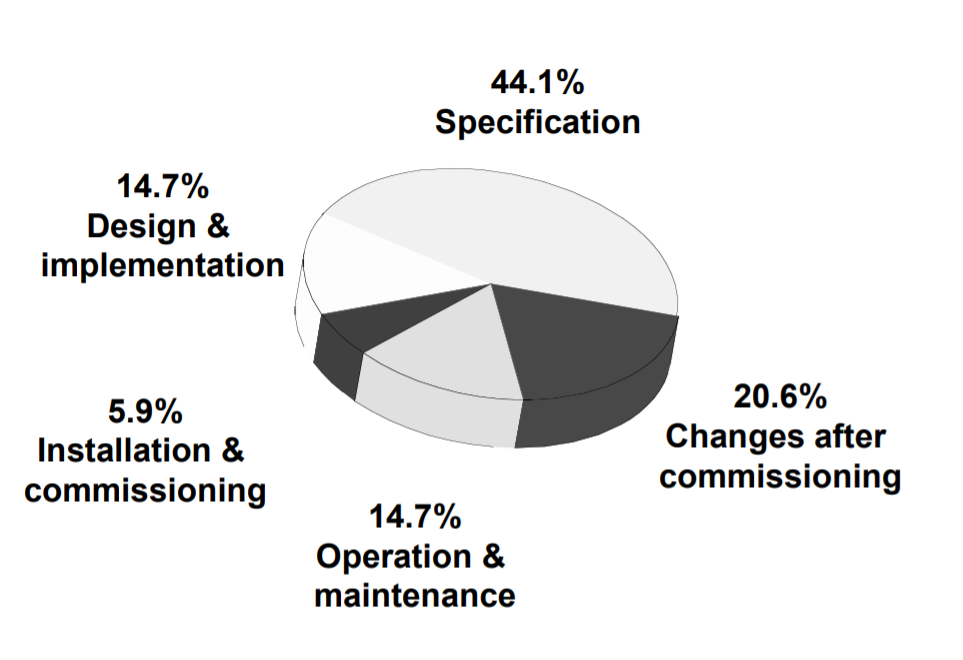
\includegraphics[scale=.33]{61508_SysFail.png}}
\caption{Main control system failure causes \cite{bell_introduction_nodate}}
\label{safety_graph}
\end{figure}

\subsection{ISO 13849}

Similar to IEC 61508, but not derived from it is the standard ISO 13849, which actually is derived from an European standard EN 954, which is already out of date. This standard mainly specifies the requirements for the design and implementation of machinery SRCS (Safety Related parts of Control Systems).

ISO 13849 is a B1 standard, which means it is a generic safety standard, which deals with one or more particular safety aspects (e.g. safety distances, surface devices, pressure sensitive devices, guards and so on). Specifically, ISO 13849 deals with electromagnetic and complex electronics, where as non-electrical technology is excluded in this standard.

It functions by estimating a level of risk reduction required for each SECS, but validation and the overall solution requires knowledge of the protective devices. ISO 13849 has 5 categories in alphabetical order, which are basing a machinery by average possibility of dangerous failure per hour \cite{ISO_13849}:

\begin{itemize}
    \item Performance Level A is $\smash{\geq 10^{-5} \: \textrm{to} < 10^{-4}}$
    \item Performance Level B is $\smash{\geq 3 \times 10^{-6} \: \textrm{to} < 10^{-5}}$
    \item Performance Level C is $\smash{\geq 10^{-6} \: \textrm{to} < 3 \times 10^{-6}}$
    \item Performance Level D is $\smash{\geq 10^{-7} \: \textrm{to} < 10^{-6}}$
    \item Performance Level E is $\smash{\geq 10^{-8} \: \textrm{to} < 10^{-7}}$
\end{itemize}

Hence, this standard focuses more on the amount of failures, estimating the required safety application for each machinery.

\section{Advantages of Functional Safety}

Safety in any application, whether its a machinery in a factory, or a product in users hands, is a mandatory requirement, functional safety is not an exception. It ensures, that physical world assets would not be in danger from Operational Technology and Informational Technology would not be in threat of unwanted actions, and in this day and age, where technology is continuously getting complex, it is not an easy task.

When Functional Safety is achieved, it is unnoticed, all of the devices and machines are functioning as intended, hence one of the advantages is intended functionality, since when functional safety fails, undesired and at some cases devastating outcome can arise, especially if the device or machine in question handles a lot of force, is crucial for quality of life and so on.

\section{Disadvantages of Functional Safety}

It is important to derive many variables in the term of safety, since this topic is already a very broad matter and as mentioned before, Functional Safety itself became too broad of a term, which requires to be separated into even smaller sub-categories, since the technology already is at a state, where one set of requirements is not as applicable for all fields of the safety related systems.

Standards is another issue, while it creates a solution for ensuring, that safety related systems would function as intended and that it would be easier for industries to follow up with the requirements, the amount of standards is increasing. Some are taking a narrow scope, some are very broad, some are just standards to be a part of another few standards. In order to understand and follow up in the subject of Functional Safety, a person has to have a lot of knowledge and expertise in this field and keep himself constantly informed, since standards also change, new additions are released and so on.

Overall, the complexity of Functional Safety is one of the disadvantages, since it is a field, which already requires systematic change and improvement, but adding to the subject more standards and requirements can make matters more complex, rather than easier to apply and safe. One of the studies, which were referenced before, which stated, that most failures comes from specifications, hence the verdict, is to focus on reviewing the product in each lifecycle phase, but on the other hand, this makes the process even more complex and time consuming.

\section{Summary and Conclusion}

All in all, the subject of safety is a very important aspect, which needs to be discussed, re-engineered when needed and expanded upon, Functional Safety is a big part of the subject. Gladly, this subject is a consideration in many industries, but the constant complexity growth of the subject shows, that the field of Functional Safety requires constant demand, since there are many various devices and machines, which could cause devastating results, if a slight overlook or miscalculation would happen.

\section{Affidavit}
I, Vytaras Juraska, herewith declare that I have composed the present paper and work by our self and without use of any other than the cited sources and aids. Sentences or parts of sentences quoted literally are marked as such; other references with regard to the statement and scope are indicated by full details of the publications concerned. The paper and work in the same or similar form has not been submitted to any examination body and has not been published. This paper was not yet, even in part, used in another examination or as a course performance.

\bibliography{references}

\end{document}
